\documentclass[a4paper]{report}
\usepackage[T1]{fontenc}%per rappresentare i font italiani, come le lettere accentate, con la giusta spaziatura
\usepackage[utf8]{inputenc}%per poter inserire nel testo .tex i caratteri unicode8
\usepackage[italian]{babel}%per poter effettuare la giusta sillabazione della lingua italiana
\usepackage{amsmath}%per poter rappresentare ed utilizzare al meglio gli ambienti e le formule matematiche
\usepackage{amssymb}%per rappresentare alcuni simboli particolari matematici
\usepackage{amsthm}%per definire e poter effettuare le dimostrazioni matematiche
%\usepackage{amsfont}%per poter avere i font matematici
\usepackage{booktabs}%per la corretta gestione delle tabelle
\usepackage{graphics}%per effettuare i grafici
\usepackage{pgfplots}%per i grafici
\usepackage{rotating}%per effettuare le rotazioni delle immagini e grafici
\usepackage{microtype}%per effettuare un aggiustamento della spaziatura tra caratteri e del font
%\usepackage{pygmentize}%Package necessario per far funzionare minted
\usepackage{minted}
\usepackage{url}%per poter rappresentare gli url nel testo latex
%\usepackage{hypertext}%per effettuare un collegamento con una pagina internet
\newtheorem{defi}{Definizione}%Definizione per avere la gestione delle definizioni
\newtheorem{prop}{Proposizione}[chapter]
\newtheorem{lem}{Lemma}
\newtheorem{teorema}{Teorema}[chapter]
\newtheorem{corol}{Corollario}[chapter]
\newtheorem{esempio}{Esempio}

\begin{document}
%Intestazione e indice dei contenuti
\title{Linguaggi di Programmazione}
\author{Marco Natali}
\date{}%rappresenta la data di compilazione del file
\maketitle

\tableofcontents

\chapter{Introduzione ai Paradigmi di Programmazione}
Nel corso di Linguaggi di Programmazione ci occupiamo di 3 importanti paradigmi di 
di linguaggi quali i linguaggi logici, linguaggi funzionali e linguaggi predicativi.

Durante il corso, e soprattutto durante la vita futura lavorativa, si devono rispettare le regole
standard di formattazione dei programmi come le regole google, regole gnu ed ecc... ossia nei programmi
devono essere rispettate le seguenti regole:
\begin{itemize}
\item usare Emacs come editor in quanto indenta lui al meglio
\item le linee di codice non devono essere più lunghe di 80 colonne
\item inserire spazi tra gli operatori e uno spazio dopo , e ; ossia 2 + 3 e (4, 5)
\item non inserire uno spazio tra il nome di una funzione/predicato e le parentesi ossia foo(4)
\item inserire uno spazio tra un istruzione di controllo e logica  e le parentesi ossia if (4 || 5)
\item non usare i commenti all'interno di un box perchè difficilmente mantenibile
\end{itemize}
I linguaggi di programmazione vengono classificati in base a dei paradigmi, ossia un modello di riferimento
su come strutturare un programma, al fine di facilitare l'apprendimento di linguaggi similari:
\begin{itemize}
\item Imperative Languages: linguaggi basati sull'architettura di Von Neumann, base di tutti i calcolatori moderni,
      in cui il processore ha il compito di leggere e scrivere le celle di memoria durante l'esecuzione della computazione.\newline
      Questa tipologia di linguaggi utilizza uno stile prescrittivo, ossia i programmi iterativi specificano una sequenza
      di istruzioni da eseguire per modificare lo stato del sistema e questo flusso può essere modificato soltanto con
      le strutture di controllo.
      Fanno parte di questo paradigma il C/C++, i linguaggi Assembler, Pascal, Python, ...
\item Logic Languages: linguaggi in cui un programma è una deduzione logica ossia ogni istruzione è una formula del linguaggio
      e noi interroghiamo il sistema per sapere se una formula del linguaggio fa parte della conoscenza rappresentata nel programma;
      questo paradigma viene utilizzato per la dimostrazione della correttezza di un programma, per rappresentare i database
      ed infine sta avendo un notevole utilizzo ultimamente nel campo dell'AI(Artificial Intelligence).
      Fa parte di questo paradigma principalmente solo il Prolog e i suoi derivati.
\item Functional Languages: linguaggi in cui il concetto di funzione è l'unica cosa importante per cui i programmi definiscono
      funzioni e l'esecuzione consiste nell'applicazione di uno o più funzioni agli argomenti.
      Fanno parte di codesto paradigma i linguaggi Lisp, Common Lisp, Scheme, Javascript, ML, Ocaml, Haskell, R, ...
\end{itemize}
Ogni dei seguenti paradigmi può avere la presenza di linguaggi object oriented, come Java, C++, Comon Lisp, Python, ...,
infatti il paradigma ad oggetti è ortogonale alla definizione dei seguenti paradigmi, anche se presume alcune features tipiche
dei linguaggi imperativi.

\section{Paradigma Imperativo}
Il paradigma imperativo, come già visto durante la definizione dei diversi paradigmi, si occupa di eseguire una sequenza di istruzioni
per effettuare la computazione infatti il paradigma imperativo è stato inventato più per la computazione ``numerica'' rispetto agli
altri paradigmi.

La struttura del programma è composta da due componenti, una per rappresentare le strutture dati e l'altra per gli algoritmi:
\begin{itemize}
\item dichiarazione: istruzioni in cui vengono dichiarate le variabili, i tipi e le funzioni necessarie per effettuare
  la computazione, ossia vengono definite le strutture dati necessarie per eseguire la computazione voluta.
\item definizione: istruzioni in cui vengono implementati gli algoritmi, per eseguire correttamente la computazione, attraverso
  l'utilizzo di istruzione facenti parte del linguaggio.
\end{itemize}

%Inserire esempio di Programma Imperativo

\section{Paradigma Logico}
La necessità di gestire le applicazione ad un maggiore livello di astrazione e di scrivere programmi il più concisi possibile ha spinto
alla creazione di nuovi paradigmi, come quello logico che analizzeremo ora.

Il paradigma logico non è più basato sull'architettura di Von Neumann ma su concetti matematici, come la logica matematica,
ed utilizza uno stile di programmazione descrittivo, ossia viene definito cosa fa parte e cosa no del problema da rappresentare.

Inoltre nella programmazione logica non è presente alcuna separazione netta tra gli algoritmi e le strutture dati e, come già
visto nella separazione tra i vari paradigmi, un programma consiste nel descrivere un problema come una serie di sentenze del linguaggio
ed interrogare il sistema, il quale effettua una deduzione sulla base della conoscenza rappresentata.

Un esempio di programma logico è il seguente:
%Inserisci file employees.pl


\section{Paradigma Funzionale}
Il paradigma funzionale, come visto nel paradigma logico, viene usato per una programmazione simbolica, è basata su concetti matematici,
adotta solitamente uno stile descrittivo di programmazione ed infine non vi è una completa separazione tra strutture dati ed algoritmi.

Il concetto fondamentale di questo paradigma è la funzione, che è una relazione tra due insiemi che associa un elemento del dominio uno e
un solo elemento del codominio.

Dopo che è stata definita una funzione, possiamo applicarla su un elemento del dominio per ottenere un valutazione della funzione per cui
un programma funzionale si riduce alla valutazione di una funzione per ottenere un valore, in cui in un linguaggio funzionale puro esso è
determinato soltanto dalla funzione e non da i valori in memoria.\newline
Questa assenza di effetti dati dalla memoria consiste nel definire una variabile come una costante matematica ossia il valore non è mutabile
a differenza delle variabili nei linguaggi imperativi che sono una astrazione di una locazione in memoria.

Un programma funzionale, come già visto nella definizione dei vari paradigmi, consiste nella definizione di un insieme di funzioni,
eventualmente ricorsive, e l'esecuzione di un programma consiste nell'applicazione di una funzione agli argomenti.

Esempio di programma funzionale:

\section{Richiami sugli ambienti RunTime e architettura degli elaboratori}
Per eseguire un programma in un qualsiasi linguaggio il sistema (ovvero il sistema operativo) deve mettere a disposizione
un ambiente \textit{run time}, che può essere anche una macchina virtuale, il quale fornisce almeno due funzionalità:
\begin{itemize}
\item mantenimento dello stato della computazione (program counter, limiti di memoria etc)
\item gestione della memoria disponibile (fisica e virtuale)
\end{itemize}

La gestione della memoria avviene usando due aree concettualmente ben distinte con funzioni diverse:
\begin{itemize}
\item lo \textit{Stack}  serve per la gestione delle chiamate (soprattutto ricorsive) a procedure, metodi, funzioni etc...(record di attivazione).
\item lo \textit{Heap} serve per la gestione di strutture dati dinamiche (liste, alberi etc...)
\end{itemize}
I linguaggi logici e funzionali (ma anche Java) utilizzano pesantemente lo Heap dato che forniscono come strutture dati built-in 
liste e spesso vettori di dimensione variabile.

La gestione dei record di attivazione è stata affrontata nei corsi di Programmazione ed Architettura, a cui si può consultare i
libri e gli appunti per rinfrescare la memoria.

La gestione della memoria, in particolare quella dinamica, può avvenire in maniera automatica, attraverso il \emph{Garbage Collector} che è
usato da Python, Java, Lisp, Prolog ed altri, oppure in maniera manuale, come in C/C++ attraverso i comandi malloc(new) e free(delete).

\chapter{Ripasso Logica Proposizionale e Predicativa}
Effettuiamo ora un ripasso della logica proposizionale e predicativa, affrontata nel corso Fondamenti dell'Informatica, al fine di rivedere
e perfezionare i concetti di logica necessari per la comprensione e la scrittura di programmi logici.

Partiamo con l'esempio di una semplice dimostrazione geometrica effettuata con le regole della logica:
\begin{teorema}
  Dato un triangolo isoscele (con $\overline{AB}=\overline{BC}$) si ha che $\angle A$, ovvero l'angolo in $A$,
  e $\angle C$, ovvero l'angolo in $C$, sono uguali.
\begin{center}
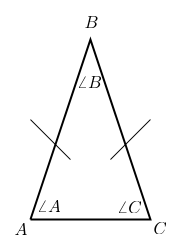
\includegraphics[scale=0.5]{img/tri.png}
\end{center}
\end{teorema}
\begin{proof}
Si comincia la dimostrazione con l'elenco delle conoscenze pregresse: 
\begin{enumerate}
\item se due triangoli sono uguali essi hanno lati e angoli uguali
\item se due triangoli hanno due lati e l'angolo sotteso uguale allora i due triangoli sono uguali
\item se viene definita la bisettrice di $\angle B$, $\overline{BH}$, si ha che $\angle ABH = \angle HBC$
\begin{center}
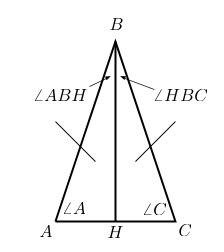
\includegraphics[scale=0.5]{img/tri2.png}
\end{center}
\end{enumerate}
Procediamo ora coi passi della dimostrazione:
\begin{enumerate}
\item $\overline{AB}=\overline{BC}$ per ipotesi
\item $\angle ABH = \angle HBC$ per la terza conoscenza pregressa
\item $\triangle HBC = \triangle ABH$ per la seconda conoscenza pregressa in quanto due lati sono uguali per ipotesi e dal passo precedente
      l'angolo sotteso ai due lati uguali è uguale in ambedue i triangoli.
\item $\angle A= \angle C$ per la prima conoscenza pregressa dato che $\triangle HBC = \triangle ABH$ 
\end{enumerate}
Siamo così giunti alla fine della dimostrazione ma adesso vogliamo rappresentarla attraverso gli strumenti della logica al fine di rendere
totalmente formale la dimostrazione per cui si effettua i seguenti passaggi:
\begin{itemize}
\item si è trasformata la seconda conoscenza pregressa in:\newline
  \textbf{se} $\overline{AB}=\overline{BC}$ \textbf{e} $\overline{BH}=\overline{BH}$ \textbf{e} $\angle ABH = \angle HBC$
  \textbf{allora} $\triangle ABH=\triangle HBC$
\item si è trasformata la prima conoscenza pregressa in:\newline
  \textbf{se} $\triangle ABH=\triangle HBC$ \textbf{allora} $\overline{AB}=\overline{BC}$ \textbf{e} $\overline{BH}=\overline{BH}$
  \textbf{e} $\overline{AH}=\overline{HC}$ \textbf{e} $\angle ABH = \angle HBC$ \textbf{e} $\angle AHB = \angle CBH$ \textbf{e} $\angle A=\angle C$
\end{itemize}
Possiamo ora procedere col processo di formalizzazione, ossia il processo che ci permette di affermare
$\overline{AB} = \overline{BC} \vdash \angle A = \angle C$ con $\vdash$ simbolo di derivazione logica, che significa consegue, allora, ecc...

Assumendo $P = \{ \overline{AB} = \overline{BC}, \angle ABH = \angle HBC, \overline{BH} = \overline{BH} \}$
ed avendo le seguenti conoscenze pregresse:
\begin{enumerate}
\item $\overline{AB}=\overline{BC} \land \overline{BH}=\overline{BH} \land \angle ABH = \angle HBC \rightarrow \triangle ABH=\triangle HBC$
\item  $\triangle ABH=\triangle HBC \rightarrow \overline{AB}=\overline{BC} \land \overline{BH}=\overline{BH} \land \overline{AH}=\overline{HC}
        \land \angle ABH = \angle HBC \land \angle AHB = \angle CBH \land \angle A=\angle C$.
\end{enumerate}
per ottenere $\overline{AB} = \overline{BC} \vdash \angle A = \angle C$ bisogna effettuare la seguente catena:
\begin{enumerate}
\item \textbf{P1:} $\overline{AB}=\overline{BC}$ preso da \textbf{P}
\item \textbf{P2:} $\angle ABH = \angle HBC$ preso da \textbf{P}
\item \textbf{P3:} $\overline{BH}=\overline{BH}$ preso da \textbf{P}
\item \textbf{P4:} $\overline{AB} = \overline{BC} \land \overline{BH} = \overline{BH} \land \angle ABH = \angle HBC$ preso da \textbf{P1, P2, P3} e       dalla regola \textbf{introduzione della congiunzione}.
\item \textbf{P5:} $\triangle ABH = \triangle HBC$ da \textbf{P4}, dalla \textbf{regola 2}  e dalla regola di inferenza detta \textbf{modus ponens}.
\item \textbf{P6:} $\overline{AB} = \overline{BC} \land \overline{BH} = \overline{BH} \land \overline{AH} = \overline{HC} \land
  \angle ABH = \angle HBC \land \angle AHB = \angle CBH \land \angle A=\angle C$ da \textbf{P5}, dalla \textbf{regola 1} e dalla regola
  \textbf{modus ponens}.
\item \textbf{P7:} $\angle A=\angle C$ da \textbf{P6} e dalla regola d'inferenza eliminazione della congiunzione 
\end{enumerate}
Abbiamo così dimostrato tutto anche per mezzo dei costrutti della logica
\end{proof}
\begin{defi}
Una dimostrazione del tipo \textit{F è conseguenza di S}, \textbf{dim}, si indica con:
$$S\,\,\vdash\,\, F$$
ed è una sequenza:
$$dim=<P_1,P_2,...,P_n>$$
con:
\begin{itemize}
\item $P_n=F$
\item $P_i \in S$ o con $P_i$ ottenibile dalle $P_1,...,P_{i-1}$ applicando una regola di inferenza
\end{itemize}
\end{defi}
Un insieme di regole di inferenza costituisce la base di un calcolo logico, il quale ha lo scopo di manipolare le formule in modo
unicamente sintattico al fine di stabilire una connessione tra un insieme di formule di partenza, dette assiemi e un insieme di conclusioni.

\subsection{Logica Proporzionale}
La logica proposizionale si occupa delle conclusioni che si possono trarre da un insieme di proposizioni, che definiscono sintatticamente la logica
proposizionale, ma purtroppo è un linguaggio limitato che non si può generalizzare le proposizioni.

La sintassi di un linguaggio è composta da una serie di formule ben formate($FBF$) definite induttivamente nel seguente modo:
%definizione formule ben formate
\begin{enumerate}
  \item Le costanti e le variabili proposizionali $\in FBF$(chiamate atomi o letterali).
  \item Se $A$ e $B \in FBF$ allora $(A \land B)$,$(A \lor B)$,$(\neg A)$,$(A \rightarrow B)$,
        $(A \iff B)$,$TA$ e $FA$ sono delle formule ben formate.
  \item nient'altro è una formula
\end{enumerate}

Esempio:\newline
$(P \land Q) \in Fbf$  è una formula ben formata\newline
$(PQ \land R) \not \in Fbf$ in quanto non si rispetta la sintassi del linguaggio definita.\newline

La semantica di una logica consente di dare un significato e un interpretazione alle formule del Linguaggio.\newline
\begin{defi}
  Sia data una formula proposizionale $P$ e sia ${P_1,\dots,P_n}$, l'insieme degli atomi che compaiono nella formula $A$.
  Si definisce come \emph{interpretazione} una funzione $v:\{P_1,\dots,P_n\} \mapsto \{T,F\}$ che attribuisce un valore di verità
  a ciascun atomo della formula $A$.
\end{defi}
I connettivi della Logica Proposizionale hanno i seguenti valori di verità:
%Tabella di Verità degli operatori
$\begin{array}{ccccccc}
\toprule
\text{A} & \text{B} & A \land B & A \lor B & \neg A & A \Rightarrow B & A \iff B \\
\midrule
    F & F & F & F & T & T & T \\
    F & T & F & T & T & T & F \\
    T & F & F & T & F & F & F \\
    T & T & T & T & F & T & T \\
\bottomrule
\end{array}$\newline

La tavola di verità costituisce la semantica di un insieme di proposizioni mentre un calcolo logico dice come generare nuove formule logiche,
ovvero espressioni sintattiche, a partire dagli assiomi e questo processo di generazione si chiama dimostrazione.

Per ottenere nuove formule dagli assiomi si usa il calcolo proposizionale, che si base su regole di inferenza, ossia regole attraverso
i quali si può derivare una nuova formula ben formata.\newline
Le regole di inferenza analizzate sono le seguenti:
\begin{esempio}[Modus Ponens]
$$\frac{a\to b,\,\,a}{b}$$
\end{esempio}

\begin{esempio}[Modus Tollens]
$$\frac{a\to b, \neg b}{\neg a}$$
\end{esempio}

\begin{esempio}[Eliminazione e Introduzione di $\land$]
$$\frac{P_1\land P_2 \land ... \land P_n}{P_i}\,\,[\mbox{Eliminazione di }\land]$$
\end{esempio}

\begin{esempio}
$$\frac{P_1, P_2,...,P_n}{P_1\land P_2 \land ... \land P_n}\,\,[\mbox{Introduzione di }\land]$$
\end{esempio}

\begin{esempio}[Introduzione di $\lor$]
$$\frac{a}{a \lor b}$$
\end{esempio}

\begin{esempio}
Ecco altre regole utili:
\begin{itemize}
\item \textbf{Terzo Escluso:}
$$\frac{a \lor \neg a}{vero}$$
\item \textbf{Eliminazione di} $\neg$:
$$\frac{\neg \neg a}{a}$$
\item \textbf{Eliminazione di} $\land$:
$$\frac{a \land vero}{a}$$
\item \textbf{Contraddizione:}
$$\frac{a \lor \neg a}{b}$$
ovvero da una contraddizione posso trarre qualsiasi conseguenza
\end{itemize}
\end{esempio}
Queste regole di inferenza fanno parte del calcolo naturale, detto anche di Gentzen, similare al calcolo tramite Tableaux visto nel corso
di Fondamenti dell'informatica.\newline
Questo tipo di calcolo consiste nel formalizzare i modi di derivare conclusioni a partire dalle premesse, ovvero di derivare direttamente un FBF
mediante una sequenza di passi ben codificati.
La regola del modus ponens  insieme al principio del terzo escluso, posso essere usati anche procedendo per assurdo alla dimostrazione
di una data formula e ciò viene detto \emph{principio di risoluzione}, affrontata poi quando analizziamo il linguaggio Prolog.


Una formula nella logica proposizionale può essere di tre diversi tipi:
%Tipologie di formule
\begin{description}
    \item[valida o tautologica]: la formula è soddisfatta da qualsiasi valutazione della Formula
    \item[Soddisfacibile non Tautologica]:la formula è soddisfatta da qualche valutazione
                        della formula ma non da tutte.
    \item[falsibicabile]:la formula non è soddisfatta da qualche valutazione della formula.
    \item[Contraddizione]:la formula non viene mai soddisfatta
\end{description}

\begin{teorema}
$A$ è una formula valida se e solo se $\neg A$ è insoddisfacibile.
$A$ è soddisfacibile se e solo se $\neg A$ è falsibicabile
\end{teorema}

Si definisce \emph{modello}, indicato con $M \models A$, tutte le valutazioni booleane
che rendono vera la formula $A$.
Si definisce \emph{contromodello}, indicato con , tutte le valutazioni booleane
che rendono falsa la formula $A$.

La logica proposizionale è decidibile, ossia posso sempre verificare il significato di una formula, infatti esiste
una procedura effettiva che stabilisce la validità o no di una formula, o se questa ad esempio è una tautologia.
In particolare il verificare se una proposizione è tautologica o meno è l’operazione di decibilità principale che si svolge
nel calcolo proposizonale.

\begin{defi}
    Se $M \models A$ per tutti gli $M$, allora $A$ è una tautologia e si indica $\models A$
\end{defi}

\begin{defi}
    Se $M \models A$ per qualche $M$, allora $A$ è soddisfacibile
\end{defi}

\begin{defi}
Se $M \models A$ non è soddisfatta da nessun $M$, allora $A$ è insoddisfacibile
\end{defi}

Una dimostrazione di una formula di una logica può venire tramite:
\begin{itemize}
  \item  \textbf{Metodo diretto}: Data un'ipotesi, attraverso una serie di passi
          si riesce a dimostrare la correttezza della Tesi
  \item \textbf{Metodo per assurdo}(non sempre accettato in tutte le logiche):
        Si nega la tesi ed attraverso una serie di passi si riesce a dimostrare
        la negazione delle ipotesi.
\end{itemize}

\begin{teorema}
    Un apparato deduttivo $R$ è completo se, per ogni formula $A \in Fbf$, $\vdash A$
    implica $\models A$
\end{teorema}

\begin{teorema}
    Un apparato deduttivo $R$ è corretto se, per ogni formula $A \in Fbf$, $\models A$
    implica $\vdash A$
\end{teorema}

\subsection{Logica del primo ordine}
La logica del primo ordine, chiamata anche logica predicativa, permette di quantificare i vari fatti ed introduce il concetto di funzione e
predicato per poter esprimere delle proprietà su una serie di individui.

Un linguaggio predicativo $L$ è composto dai seguenti insiemi di simboli:
\begin{enumerate}
    \item insieme di variabili individuali(infiniti) $x,y,z,\dots$
    \item connettivi logici $\land \lor \neg \rightarrow \iff$
    \item quantificatori  $\forall \exists$
    \item simboli ( , )
    \item Costanti proposizionali $T,F$
    \item simbolo di uguaglianza $=$, eventualmente assente
\end{enumerate}
Questa è la parte del linguaggio tipica di ogni linguaggio del primo ordine poi
ogni linguaggio definisce la propria segnatura ossia definisce in maniera autonomo:
\begin{enumerate}
    \item insiemi di simboli di costante $a,b,c,\dots$
    \item simboli di funzione con arieta $f,g,h,\dots$
    \item simboli di predicato $P,Q,Z,\dots$ con arietà
\end{enumerate}

%Esempio
Esempio:Linguaggio della teoria degli insiemi \newline
Costante:$\emptyset$\newline
Predicati:$\in(x,y)$, $=(x,y)$

Esempio:Linguaggio della teoria dei Numeri \newline
Costante:$0$ \newline
Predicati:$<(x,y)$,$=(x,y)$ \newline
Funzioni:$succ(x)$,$+(x,y)$,$*(x,y)$

%Definizione di Termini e Formule ben formate
Per definire le formule ben formate della logica predicativa bisogna prima definire
l'insieme di termini e le formule atomiche.

\begin{defi}
    L'insieme $TERM$ dei termini è definito induttivamente come segue
    \begin{enumerate}
        \item Ogni variabile e costante sono dei Termini
        \item Se $t_1 \dots t_n$ sono dei termini e $f$ è un simbolo di funzione di arietà $n$
              allora $f(t_1,\dots,t_n)$ è un termine
    \end{enumerate}
\end{defi}

\begin{defi}
    L'insieme $ATOM$ delle formule atomiche è definito come:
    \begin{enumerate}
        \item $T$ e $F$ sono degli atomi
        \item Se $t_1$ e $t_2$ sono dei termini, allora $t_1 = t_2$ è un atomo
        \item Se $t_1,\dots,t_n$ sono dei termini e $P$ è un predicato a $n$ argomenti,
              allora $P(t_1,\dots,t_n)$ è un atomo.
    \end{enumerate}
\end{defi}

\begin{defi}
    L'insieme delle formule ben formate($FBF$) di $L$ è definito induttivamente come
    \begin{enumerate}
        \item Ogni atomo è una formula
        \item Se $A,B \in FBF$, allora $\neg A$, $A \land B$,$A \lor B$,$A \rightarrow B$
              e $A \iff B$ appartengono alle formule ben formate
        \item Se $A \in FBF$ e $x$ è una variabile, allora $\forall x A$ e $\exists x A$
              appartengono alle formule ben formate
        \item Nient'altro è una formula
    \end{enumerate}
\end{defi}

%Variabili legate e chiuse
\begin{defi}
    L'insieme $var(t)$ delle variabili di un termine $t$ è definito come segue:
    \begin{itemize}
        \item $var(t) = \{t \}$, se $t$ è una variabile
        \item $var(t) = \emptyset$ se $t$ è una costante
        \item $var(f(t_1,\dots,t_n)) = \bigcup _{i = 1} ^n var(t_i)$
        \item $var(R(t_1,\dots,t_n)) = \bigcup _{i = 1} ^ n var(t_i)$
    \end{itemize}
\end{defi}

%Termini chiusi ed aperti
Si definisce come \emph{aperto} un termine che non contiene variabili altrimenti
si definisce il termine come \emph{chiuso}.\newline
Le variabili nei termini e nelle formule atomiche possono essere libere
in quanto gli unici operatori che "legano" le variabili sono i quantificatori.

Il campo di azione dei quantificatori si riferisce soltanto alla parte in cui
si applica il quantificatore per cui una variabile si dice \emph{libera}
se non ricade nel campo di azione di un quantificatore altrimenti la variabile si dice \emph{vincolata}.

Si aggiunge una nuova regola d'inferenza per la logica dei predicati, l'eliminazione del quantificatore universale $\forall$:
$$\frac{\forall x, T(...,x,...), c\in C}{T(...,c,...)}$$

Abbiamo altre regole di inferenza per il quantificatore esistenziale:
\begin{itemize}
\item Introduzione del quantificatore esistenziale $\exists$:
$$\frac{T(...,c,...), c\in C}{\exists x, T(...,x,...)}$$
\item si hanno le seguente identità:
$$\exists x, \neg T(...,x,...)\equiv \neg\forall x, T)...,x,...)$$
$$\forall x, \neg T(...,x,...)\equiv \neg\exists x, T(...,x,...)$$
\end{itemize}

\chapter{Prolog:Programmazione Logica}
Dopo aver effettuato un ripasso della logica, incominciamo a considerare il Prolog e la programmazione logica:
le basi del PROLOG (PROgramming in LOGic) sono state poste da Robert Kowalski e Marten Van Emdem, mentre la sua progettazione e implementazione,
avvenuta nel 1972 a Marsiglia attraverso Alain Colmerauer e Philippe Roussel.

Si tratta di un linguaggio di programmazione logica basato sulle Clausole di Horn, ovvero un insieme di procedure attivate
da una asserzione iniziale d’obiettivo e la procedura utilizzata da prolog per la computazione è il principio di risoluzione.

Un programma prolog è un formato da un insieme di istruzioni, rappresentanti un sottoinsieme di frasi ben formate della logica del primo ordine
e il sistema prolog ha il fine di determinare se una data assunzione è verificata o meno nel programma e sotto quali eventuali vincoli
ciò risulta  verificato.

I componenti basilari di un programma prolog, rappresentanti tutti una clausola di Horn, sono:
\begin{description}
\item [Fatti]: indica una relazione esistente tra due oggetti, che può venire chiama predicato.
               \begin{minted}{prolog}
                 worksFor(paolo, coop).
               \end{minted}
\item [Query]: chiede al sistema se una relazione esiste tra gli oggetti e quindi inizia una deduzione per stabilire se la query
               è una conseguenza diretta del programma, dopo l'applicazione del modus ponens universale per un numero finito di volte.
               \begin{minted}{prolog}
                 :- worksFor(paolo, trenord).
               \end{minted}
 
\item [Regole]: definisce una nuova relazione esistente tra gli oggetti, ossia permette di derivare una nuova conclusione
                da una serie di fatti e regole.
                \begin{minted}{prolog}
                  parent(X, Y) :- father(X, Y).
                \end{minted}
                la testa della regola $A$, viene detta conseguenza mentre il corpo $B_1, B_2, \dots, B_n$ sono l'antecedente
                e il simbolo $:-$ indica il simbolo logico di implicazione.\newline
                Una relazione può essere definita ricorsiva, e in questo caso necessita di due regole, una per il caso base e
                una per il caso passo.
                
\end{description}
I fatti e le regole sono quantificate universalmente mentre una query si intende sempre quantificata esistenzialmente, per cui una query
risponde true se esiste un instanza $\alpha$ che verifica la query altrimenti risponde false.

Le query e le regole le abbiamo definite nella forma generale, ossia possiamo definire regole e query su congiunzioni di termini,
infatti il simbolo ``,'' rappresenta l'operatore logico and, perciò in caso più termini hanno lo stesso simbolo di variabile
l'instanza $\alpha$ deve essere la stessa per stabilire se una query è una conseguenza diretta del programma.

Le regole stabiliscono una relazione di implicazione, indicato con il simbolo :-, infatti definiamo che risulta A se risulta verificato
B_1, B_2, $\dots$, B_n, ovviamente sempre dal punto di vista sintattico.
Per vedere al meglio questo concetto di implicazione vediamo la definizione del concetto di nonno nel linguaggio Prolog:
\begin{minted}{prolog}
  grandfather(X, Y) :- father(X, Z), parent(Z, Y).
\end{minted}
Questa relazione stabilisce che X è il nonno di Y se risulta che esiste un Z tale che X è padre di Z e Z è genitore di Y.

Per riuscire a stabilire se un goals è una conseguenza diretta del programma il sistema prolog utilizza il principio di risoluzione,
utilizzato per effettuare la dimostrazione del programma , e il principio di unificazione, necessario come si evince dal nome per
unificare le variabili presenti in una formula del programma.

\subsection{Principio di Risoluzione}
Il principio di risoluzione è una regola di inferenza generalizzata semplice e facilmente implementabile in un calcolatore, assieme all'
algoritmo di unificazione, che opera su formule ben formate nella forma normale congiuntiva, in cui i letterali si chiamano clausole,
e viene utilizzata per la dimostrazione di formule ben formate attraverso la refutazione per assurdo.
La regola di inferenza ha la seguente forma:
$$\frac{p\vee r,\, s\lor r}{p\vee s}\,\,\,\,\,\,\,\,\,\,\frac{\neg r,\, r}{\perp}$$
dove:
\begin{itemize}
\item $p \lor  s$ è la \textit{clausola risolvente}
\item $\perp$ è la \textit{clausola vuota}, che corrisponde all'aver creato una contraddizione con delle FBF,ossia posso dedurre qualsiasi cosa,
       compresa anche la clausola vuota(posso infatti dedurre qualsiasi cosa, anche la clausola vuota)
\end{itemize}

vediamo un'altra regola di inferenza:
\begin{esempio}[(unit) resolution]
$$\frac{\neg p,\,\, q_1\vee q_2\vee ... \vee q_k \vee p}{q_1\vee q_2\vee ... \vee q_k}$$
o anche:
$$\frac{p,\,\, q_1\vee q_2\vee ... \vee q_k \vee \neg p}{q_1\vee q_2\vee ... \vee q_k}$$
è una regola di risoluzione molto generale, chiamata anche procedura di Davis-Putnam, e se una delle due clausole da risolvere
è un \textit{letterale} si parla di \emph{unit resolution}.\newline
Come esempio si può avere:
\begin{itemize}
\item non piove, piove e c'è il sole
\item c'è il sole
\end{itemize}
\end{esempio}

Prolog per stabilire se un goal e/o regola risulta verificata utilizza la refutazione per assurdo, ossia data una proposizione P suppone che
sia falsa ed applicando le regole di inferenza se risulta che $\neg P$ sarebbe assurdo afferma che $P$ è verificata.

Le formule del linguaggio Prolog sono \emph{clausole di Horn}, definite nelle seguenti regole.
Ogni FBF può essere in \textit{forma normale a clausola}:
\begin{itemize}
\item \textit{formula normale congiunta:} congiunzione di disgiunzioni o di negazione di predicati (sia positivi che negativi):
  \begin{equation*}
    \land_i(\lot_iL_{ij})
  \end{equation*}
\begin{esempio}
ecco degli esempi:
\begin{itemize}
\item $(p(x)\vee q(x,y)\vee \neg t(z))\wedge(p(w)\vee\neg s((u)\vee \neg r(v))$
\item $(\neg t(z))\vee (p(w)\vee\neg s(u))\wedge (p(x)\vee s(x)\vee q(y))$
\end{itemize}
che sono riscrivibili come:
$$t(z)\to p(x)\vee q(x,y)$$
e
$$s(u)\wedge r(v)\to p(w)$$
\end{esempio}
\item \textit{forma normale disgiunta}: disgiunzione di congiunzioni o di negazione di predicati (sia positivi che negativi)
  \begin{equation*}
    \lor_i(\land_i L_{ij})
  \end{equation*}
\end{itemize}
Le clausole con un solo letterale positivo solo le \textit{clausole di Horn}, con lo presenza o meno di letterali negativi,
e un programma in prolog è una collezione di \textit{clausole di Horn}.\newline
Ovviamente non tutte le formule ben formate possono rappresentate tramite le clausole di Horn per cui il Prolog è un sottoinsieme
della logica del Primo Ordine.\newline
Attraverso questa restrizione nel 1974 Kowalski produsse un interpretazione procedurale delle dimostrazione e ciò diventò la base
della semantica di ogni sistema prolog.

Ogni espressione prolog viene chiamata \emph{Termine}, che può essere della seguente tipologia:
\begin{description}
\item [atomi] : elemento base del sistema prolog e può essere rappresentato da un numero, qualsiasi sequenza racchiusa da (' '),
  una sequenza di caratteri alfanumerici, con la lettera minuscola iniziale, e nel swprolog anche una stringa indica un atomo.

\item [variabili] : sequenza di caratteri alfanumerici, iniziata con la lettera maiuscola oppure con \_ e vengono inizializzate
  quando il sistema prova a dimostrare una query.\newline
                    Una variabile composta soltanto dal simbolo \_ viene detta \emph{anonymous}.

\item [termini composti]: termine composto da un funtore, simbolo rappresentante il nome di una funzione o predicato, e da una sequenza
                          di termini all'interno di parentesi e separati da una virgola.                    
\end{description}

Un programma caricato nel sistema prolog rappresenta una base di conoscenza e questa base può venire rappresentata in vari modi:
\begin{itemize}
\item tutte le informazioni vengono rappresentate come argomenti in un'unica relazione e ciò può essere comodo solo per
  piccole relazioni dato che è difficile da mantenere e coprendere una relazione così definita.
 %Inserire esempio
\item le informazioni vengono rappresentate con più relazione annidate tra di loro e ciò aumenta la leggibilità e
  la mantenibilità del programma prolog.
 %Inserire esempio
\item tutte le relazioni possono essere rappresentate tramite lo schema XML
\end{itemize}

\section{Principio di Unificazione}
Il principio di unificazione è il cuore del modello di computazione dei programmi logici ed è alla base della deduzione automatica
e dell'uso dell'inferenza logica nell'intelligenza artificiale.

Per poter definire il principio di unificazione introduciamo le seguenti definizioni:
\begin{itemize}
  \item Un termine $t$ è un instanza comune  di $t_1$ e $t_2$ se esistono le sostituzioni $\alpha_1$ e $\alpha_2$
        che rendono $t$ uguale a $\alpha_1t_1$ e a $\alpha_2t_2$.
  \item Un termine $s$ è un termine generale del termine $t$ se $t$ è un'istanza di $s$ ma $s$ non è un istanza di $t$.

  \item Un termine $s$ è una variante alfabetica del termine $t$ se $t$ è un istanza di $s$ e $s$ è un istanza di $t$.
\end{itemize}
L'unificazione tra due termini consiste nell'effettuare una sostituzione che rende i due termini identici
per cui c'è una relazione chiusa con l'instanza comune di due termini.

Il principio di unificazione consiste nel trovare il \emph{mgu}(Most general unifier),
l'unificazione la cui instanza comune è un termine generale, e in caso non lo trova riporta un fallimento.
Presentiamo ora alcuni esempi per capire come funziona il Mgu:
\begin{minted}{prolog}
Mgu(42, 42) % ->{} non serve nessuna sostituzione
Mgu(42, X) % ->{X/42} ovvero X deve essere 42
Mgu(X,42) % ->{X/42} ovvero X deve essere 42
Mgu(foo(bar, 42), foo(bar, X)) % ->{X/42} ovvero X deve essere 42
Mgu(foo(X, 42), foo(bar, X)) % ->{Y/bar, X/42} ovvero X deve essere 42

Mgu(foo(bar(42), baz), foo(X, Y))  /* ->{X/bar (42), Y/baz}
 ovvero X deve essere  bar(42) e Y baz*/
Mgu(foo(X), foo(bar(Y))) 
Mgu(foo(bar(42), baz), foo(X, Y))  /* ->{X/bar (y), Y_:G001}
 ovvero non si ha soluzione */
\end{minted}
L'Mgu non è altro che il risultato finale della procedura di valutazione del Prolog. Il modo più semplice per vedere se l'unificazione funziona è usare "=", ovvero, ricollegandoci al codice sopra:
\begin{minted}{prolog}
?- 42 = 42.
Yes

?- 42 = X.
X = 42 % per rendere vera l'affermazione serve x = 42
Yes

?- foo(bar, 42) = foo(bar, X).
X = 42
Yes

?- foo(Y, 42) = foo(bar, X).
Y = bar
X = 42
Yes

?- foo(bar(42), baz) = foo(X, Y).
X = bar(42)
Y = baz
Yes

?- foo(X) = foo(bar(Y)).
X = bar(Y)
Y = _G001
Yes

?- foo(42, bar(X), trillian) = foo(Y, bar(Y), X).
No
\end{minted}

%Si ha quindi un solo termine come conseguente (\textit{regola di Horn}). Si ha quindi:
%\textit{un pesce è un animale e ha le squame}: 
%\begin{minted}{prolog}
%pesce(x) :- animale(x), ha_le_squame(x).
%\end{minted}
%oppure:\\
%\textit{gigi ama chiunque ami il vino}
%aggiungi prolo


Si definisce una lista in Prolog racchiudendo gli elementi (termini e/o variabili logiche) della lista tra parentesi quadre \textit{[} e \textit{]}
e separandoli da virgole. Gli elementi di una lista in Prolog possono essere termini
qualsiasi o liste. La lista vuota si indica con \textit{[]}.
Una lista non vuota si può dividere in \textit{testa} e \textit{coda}:
\begin{itemize}
\item la testa è il primo elemento della lista
\item la coda rappresenta tutto il resto ed è sempre una lista
\end{itemize}
Presentiamo ora degli esempi di liste in Prolog:
\begin{minted}{prolog}
[a, b, c] % a è la testa e [b, c] la coda
[a, b] % a è la testa e [b] la coda
[a] % a è la testa e [] la coda
[[a]] % [a] è la testa e [] la coda
[[a, b], c] % [a, b] è la testa e [c] la coda
[[a, b], [c], d] % [a, b] è la testa e [[c], d] la coda
\end{minted}
Prolog possiede uno speciale operatore usato per distinguere tra l'inizio e la coda di una lista: l'operatore \textit{|}:
\begin{minted}{prolog}
?- [X | Ys] = [mia, vincent, jules, yolanda].
X = mia
Ys = [vincent, jules, yolanda]
Yes

?- [X, Y | Zs] = [the, answer, is, 42].
X = the
Y = answer
Zs = [is, 42]
Yes

?- [X, 42 | _] = [41, 42, 43, foo(bar)].
X = 41
Yes
\end{minted}
La lista vuota \textit{[]} in prolog è gestita come una lista speciale:
\begin{minted}{prolog}
?- [X | Ys] = [].
No
\end{minted}

In Prolog la base di conoscenza è nascosta ed è accessibile solo tramite opportuni comandi o tramite ambiente di programmazione
per cui bisogna poter caricare un insieme di fatti e regole nell'ambiente Prolog, nel nostro caso SW-Prolog.
Per farlo si ha il comando \textit{consult}, che appare come un predicato da valutare (un goal) e prende almeno un termine che denota un file
come argomento, file che deve contenere fatti e regole
\begin{minted}{prolog}
?- consult(’guida-astrostoppista.pl’).
Yes

?- consult(’Projects/Lang/Prolog/Code/esempi-liste.pl’).
Yes
\end{minted}

il predicato \textit{reconsult} deve invece essere usato quando si vuole ricaricare un file (ovvero un data o knowledge base) nell'ambiente Prolog.
L’effetto è di prendere i predicati presenti nel file, rimuoverli completamente dal data base interno
e di reinstallarli utilizzando le nuove definizioni:
\begin{minted}{prolog}
?- reconsult(’guida-astrostoppista.pl’).
Yes
% A questo punto la base di dati Prolog contiene il
% nuovo contenuto del file.
\end{minted}

?- reconsult(user). % Notare il sotto-prompt.
|- foo(42).
|- friends(zaphod, trillian).
|- ^D
Yes

% A questo punto la base di dati Prolog contiene i due
% fatti inseriti manualmente.
?- friends(zaphod, W).
W = trillian
Yes
\end{minted}

Il Prolot lavora su strutture ad albero e anche i programmi sono strutture dati manipolabili con predicati \textit{extra-logici}
per cui il prolog usa la ricorsione invece dell'assegnamento.

Vediamo ora un programma che effettua la somma tra due numeri naturali:
\begin{minted}{prolog}
sum(0, X, X).
sum(s(X), y, s(Z)) -: sum(X, Y, Z).
\end{minted}
con $s(n)$ interpretato come il successore ($0=0,\, s(0)=1, \,s(s(0))=2,... $).\newline
Quando viene specificato un goal esso viene confrontato con tutte le clausole di programma, che usa il procedimento di negazione
e di trasformazione in sintassi Prolog come viene mostrato in dettaglio con questo esempio:
\begin{itemize}
\item  interroghiamo il programma:
$$\exists X\,\,\, sum(s(0),\, 0,\, X)\,\,\,\,\,\{X\,/\, s(0)\}$$
$$\exists W\,\,\, sum(s(s(0)),\, s(0), \, W)\,\,\,\,\,\{W\,/\, s(s(s(0)))\}$$
dove $\{X\,/\, s(0)\}$ e $\{W\,/\, s(s(s(0)))\}$ sono le sostituzioni che rappresentano il risultato
\item usiamo il procedimento di negazione e trasformazione in sintassi:
\begin{minted}{prolog}
:- sum(s(0), 0, N).    %{N / s(0)}
:- sum (s(s(0)), s(0), W).     %{W / s(s(s(0)))}
\end{minted}
con $\{N\, /\, s(0)\}$ e $\{W \,/\, s(s(s(0)))\}$ che sono le \textbf{sostituzioni}.

Una computazione corrisponde al tentativo di dimostrare, tramite la regola di risoluzione, che una formula segue logicamente da un programma
e si ha inoltre che si deve determinare una sostituzione per le variabili del goal per cui la query segue  logicamente dal programma:
\begin{esempio}
Sia dato il programma P e la query:
\begin{minted}{prolog}
:- p(t1, t2, ..., tm).
\end{minted}
se \textbf{X1,..., Xn} sono le variabili in \textbf{t1,..., tm}, il significato della query è:
$$\exists X1,\,..., \,Xn\, . \,p(t1, t2, ..., tm)$$
e si cerca una sostituzione:
$$s=\{X1\,/\,s1,...,\, Xn\,/\,sn$$
con gli $s\,i$ termini tali per cui:
$$P\vdash s[p(t1, t2, ..., tm)]$$
\end{esempio}
Dato un insieme di clausole di Horn è possibile derivare la clausola vuota solo se c'è almeno una clausola senza testa, ovvero una query $G_0$
, in cui si deve dimostrare che da $P \cup G_0$ si può derivare la clausola e ciò avviene per assurdo col principio di risoluzione.

Nel prossimo sottoparagrafo vediamo come effuttua la risoluzione il sistema Prolog, che per efficienza usa una forma particolare di risoluzione.
\subsection{Risoluzione ad Input Lineare (SLD)}
Il sistema Prolog dimostra la veridicità di un goal eseguendo una sequenza di passi di risoluzione, il cui ordine di esecuzione
determina sistemi di prova più o meno efficienti.\newline
In Prolog la risoluzione avviene sempre fra l’ultimo goal derivato in ciascun passo e una \emph{clausola di programma}
e questa forma è detta \emph{Risoluzione-SLD}, dove le sentenze lineari sono le clausole di Horn.
\begin{esempio}
partiamo dal goal $G_i$:
$$G_i\equiv \,\,\,?-\, A_{i,\, 1}, ...,  A_{i,\, m}.$$
e dalla regola:
$$A_r\,\,\,:-\,\,\, B_{r,\,1},..., B_{r,\,k}.$$
se esiste un unificatore $\sigma$ tale che $\sigma[A_r]=\sigma[A_{i,\,1}]$ allora si ottiene il nuovo goal:
$$G_{i+1}\equiv\,\,\,B^{'}_{r,\,1},..., B^{'}_{r,\,k},A^{'}_{i,\, 1}, ...,  A^{'}_{i,\, m}.$$
che è un passo di risoluzione eseguito dal sistema Prolog (con $\sigma[A_{i,\,m}]=A^{'}_{i,\,m}$ 4 $\sigma[B_{i,\,m}]=B^{'}_{i,\,m}$.
La scelta di unificare il primo sottogoal di $G_i$ è arbitraria infatti si sarebbe potuto scegliere un arbitario sottogoal di $G_i$.
\end{esempio}
\begin{esempio}
partiamo dal goal $G_i$:
$$G_i\equiv \,\,\,?-\, A_{i,\, 1}, ...,  A_{i,\, m}.$$
e dalla regola (ovvero dal \textbf{fatto}):
$$A_r.$$
se esiste un unificatore $\sigma$ tale che $\sigma[A_r]=\sigma[A_{i,\,1}]$ allora si ottiene il nuovo goal:
$$G_{i+1}\equiv\,\,\,A^{'}_{i,\, 2}, ...,  A^{'}_{i,\, m}.$$
che ha dimensioni minori di $G_i$ avendo $m-1$ sottogoal
\end{esempio}
Nella risoluzione SLD si possono avere i seguenti risultati:
\begin{itemize}
\item \textbf{successo:} si genera la clausola vuota, ovvero se per $n$ finito $G_n$ è uguale alla clausola vuota $G_:n\equiv\,\,\,:-$
\item \textbf{insuccesso finito}: se per $n$ finito $G_n$  non è uguale alla clausola vuota $G_:n\equiv\,\,\,:-$ e non è più possibile derivare un nuovo \textit{risolvente} da $G_n$ ed una clausola d programma
\item \textbf{successo infinito: }se è sempre possibile derivare nuovi risolventi tutti diversi dalla clausola vuota
\end{itemize}
La \textbf{sostituzione di risposta} è la sequenza di unificatori usati; applicata alle variabili nei termini del goal iniziale dà la risposta finale.\\
Durante il processo di generazione di goal intermedi si costruiscono delle varianti dei letterali e delle clausole coinvolti
mediante larinominazione di variabili infatti una variante per una clausola $C$ é la clausola $C^{'}$ ottenuta da $C$ rinominando le sue variabili
\begin{esempio}
esempio:
\begin{minted}{prolog}
p(X) :- q(X, g(Z)).
% è uguale alla clausola con variabili rinominate:
p(X1) :- q(X1, g(FooFrobboz)).
\end{minted}
\end{esempio}
Possono esserci più clausole di programma utilizzabili per applicare la risoluzione con il goal corrente ed esistono diverse strategie di ricerca:
\begin{itemize}
\item \textbf{in profondità (Depth First)}: si sceglie una clausola e si mantiene fissa questa scelta, finché non si arriva alla clausola vuota o alla impossibilità di fare nuove risoluzioni; in questo ultimo caso si riconsiderano le scelte fatte precedentemente
\item \textbf{in ampiezza (Breadth First)}: si considerano in parallelo tutte le possibili alternative
\end{itemize}
Ogni sistema di programmazione logica sceglie la propria strategia e il Prolog ha deciso di adottare una strategia di risoluzione
in profondità con Backtracking, ossia la possibilità di ritornare indietro e provare tutte le possibilità, al fine di avere così
un risparmio di memoria anche se non è una strategia completa per le clausole di Horn.

Introduciamo ora l'importante argomento degli alberi di derivazione, per analizzare come un sistema Prolog effettua la computazione
e quali passi esegue per riuscire a stabilire se una data query deriva dal programma o meno.

Dato un programma logico $P$, un goal $G_i$ e una regola di calcolo $R$ si ha che un \textit{albero SLD} per $P\cup G_i$ via $R$
è definito sulla base del processo di prova visto precedentemente:
\begin{itemize}
\item ciascun \textbf{nodo} dell'albero è un goal (possibilmente vuoto)
\item la \textbf{radice }dell'albero SLD è il goal $G_0$
\item dato il nodo: $:-\,\,\, A_1,...,A_{m-1},A_m,A_{m+1},...,A_k$
  se $A_m$ è il sottogoal selezionato dalla regola di calcolo $R$, allora questo nodo (genitore) ha un nodo figlio
  per ciascuna clausola del tipo:
$$C_i\equiv A_i\,\,\, :-\,\,\, B_{i,\,1},...,B_{i,\,q}$$
$$C_k\equiv A_k$$
di $P$ tale che $A_i$ e $A_M$ ($A_K$ e $A_m$) sono unificabili attraverso la sostituzione più generale $\sigma$.\newline
Il nodo figlio è etichettato con la clausola goal
$$:-\,\,\,\sigma[A_1,...,A_{m-1},B_{i,\,i},...,B_{i,\,q},A_{m+1},...,A_k]$$
$$:-\,\,\,\sigma[A_1,...,A_{m-1},A_m,A_{m+1},...,A_k]$$
e il ramo dal nodo padre al figlio è etichettato dalla sostituzione $\sigma$ e dalla clausola selezionata $C_i$ o $C_k$.\\
Il nuovo nodo $:-$ non ha figli.
\end{itemize}
La regola $R$ è variabile. Si ha:
\begin{itemize}
\item \textbf{regola Left-most}: ovvero si ha la scelta del sottogoal più a sinistra 
\item \textbf{regola Right-most}: ovvero si ha la scelta del sottogoal più a destra
\item si può avere la scelta di un sottogoal a caso
\item se si ha un modo per decider il miglior sottogoal  
\end{itemize}
Ogni sistema logico decide la propria modalità di applicazione della regola e il sistema Prolog utilizza sempre la regola left-most.

L'albero SLD, generato implicitamente dal sistema Prolog, ordina i figli di un nodo secondo l'ordine dall'alto verso il basso
delle regole e dei fatti del programma P. 
\begin{esempio}
Ecco un esempio:
\begin{center}
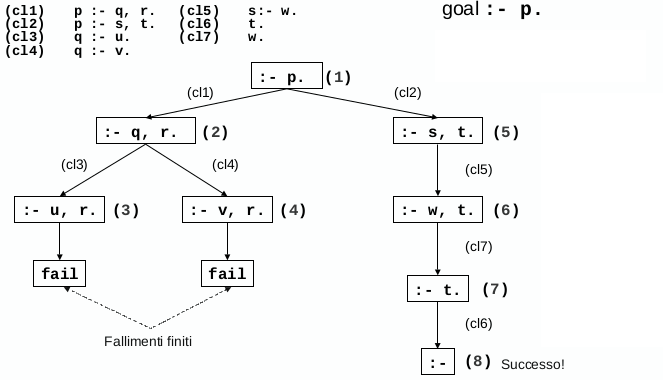
\includegraphics[scale=0.7]{img/alb.png}
\end{center}
\end{esempio}
Ad ogni ramo di un albero SLD corrisponde una derivazione SLD e ogni ramo che termina con il nodo vuoto $:-$; la regola di calcolo
influisce sulla struttura dell'albero per quanto riguarda l'ampiezza e la profondità ma tuttavia non influisce sulla correttezza e completezza.

\begin{esempio}
  Ecco un altro esempio, con fallimento infinito, dove la clausola vuota può essere generata ma il Prolog non è in grado di trovare
  questa soluzione dato che la sua strategia di percorrimento dell’albero (implicito) di soluzioni è depth-first con backtracking :
\begin{center}
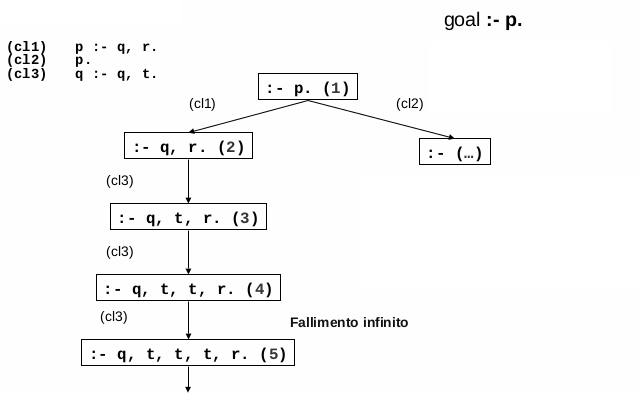
\includegraphics[scale=0.7]{img/alb2.png}
\end{center}
\end{esempio}
\begin{esempio}
%aggiungi esempio
\end{esempio}
\subsection{Cut e Backtracking}
Introduciamo ora il predicato \emph{Cut}, il quale permette di controllare il backtracking, in quanto si tagliano certe possibilità
di ritornare indietro nelle scelte durante la computazione.

Il predicato cut si indica con $!$ e il Prolog effettua un'interpretazione procedurale, sempre per il fatto che viene eseguito su un calcolatore.

Come abbiamo affermato precedentemente, le clausole nel data base di un programma Prolog vengono considerate “da sinistra, verso destra”
e “dall'alto al basso” per cui se un (sotto)goal fallisce, allora il dimostratore Prolog, sceglie un'alternativa,
scandendo “dall'alto” verso “il basso” la lista delle clausole.
Questa procedurà può venire controllata dal \textit{cut} infatti per esempio:
\begin{minted}{prolog}
a :- b1, b2, ..., bk, !, ..., bn.
\end{minted}
Questo è l'effetto del cut:
\begin{itemize}
\item se il goal corrente \textit{G} unifica con \textit{a} e $b_1,...,b_k$ hanno successo,
      allora il dimostratore si impegna inderogabilmente alla scelta di C per dimostrare G.
\item ogni clausola alternativa (successiva, in basso) per \textit{a} che unifica con \textit{G} viene ignorata
\item se un qualche $b_j$ con $j > k$ fallisse, il backtracking si fermerebbe al cut e le altre scelte sono rimosse dall'albero di derivazione
\item quando il backtracking raggiunge il cut, allora il cut fallisce e la ricerca procede dall’ultimo punto di scelta
      prima che \textit{G} scegliesse \textit{C}
\end{itemize}
%aggiungere gestione stack di prolog
vediamo un albero di derivazione in caso di cut:
\begin{center}
	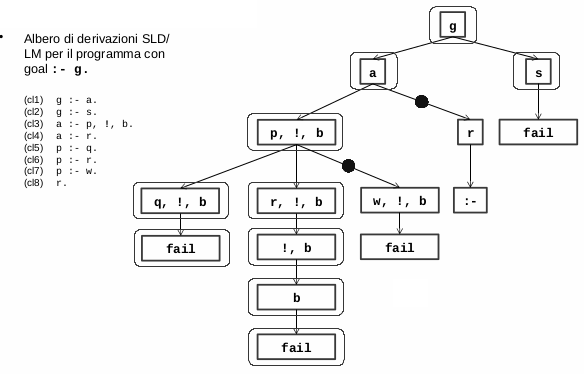
\includegraphics[scale=0.8]{img/cut.png}
\end{center}
Si hanno due tipi di cut:
\begin{itemize}
\item \textbf{green cut: } utili per esprimere “determinismo” (e quindi per rendere più efficiente il programma)
\item \textbf{red cut: } usati per soli scopi di efficienza, hanno per caratteristica principale quella di omettere
  alcune condizioni esplicite in un programma e, soprattutto, quella di modificare la semantica del programma equivalente senza cuts.
  Hanno degli effetti indesiderabili ma sono utili per cui vanno maneggiati con cura per evitare gli effetti negativi.
\end{itemize}
consideriamo il seguente codice:
\begin{minted}{prolog}
/* merge di due liste ordinate*/

merge([X | Xs], [Y | Ys], [X | Zs]) :-
	X < Y,
	merge(Xs, [Y | Ys], Zs).
merge([X | Xs], [Y | Ys], [X, Y | Zs]) :-
	X = Y,
	merge(Xs, Ys, Zs).
merge([X | Xs], [Y | Ys], [Y | Zs]) :-
	X > Y,
	merge([X | Xs], Ys, Zs).
merge([], Ys, Ys).
merge(Xs, [], Xs).

/+ minimo tra due numeri */

minimum(X, Y, X) :- X =< Y.
minimum(X, Y, Y) :- Y < X.
\end{minted}
vediamo cosa succede:
\begin{center}
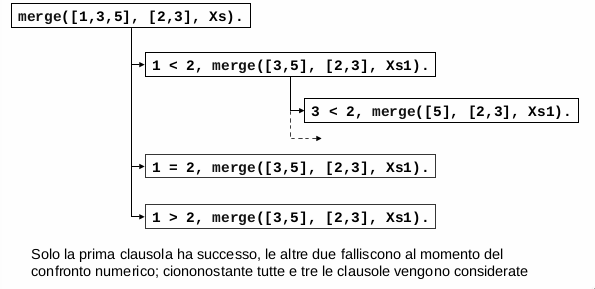
\includegraphics[scale=0.8]{img/cut2.png}
\end{center}
consideriamo la seguente query:
\begin{shaded}
\begin{lstlisting}[language=bash]
?- merge([], [], Xs).
Xs = [];
Xs = [];
False.
\end{lstlisting}
\end{shaded}
si ha una soluzione di troppo.
Un programma Prolog si dice \textbf{deterministico} quando una sola delle clausole serve (o si vorrebbe servisse) per provare un dato goal. Si usano quindi i green cuts:
\begin{minted}{prolog}
merge([X | Xs], [Y | Ys], [X | Zs]) :-
	X < Y, !,
	merge(Xs, [Y | Ys], Zs).
merge([X | Xs], [Y | Ys], [X, Y | Zs]) :-
	X = Y, !,
	merge(Xs, Ys, Zs).
merge([X | Xs], [Y | Ys], [Y | Zs]) :-
	X > Y, !,
	merge([X | Xs], Ys, Zs).
merge([], Ys, Ys) :- !.
merge(Xs, [], Xs) :- !.
\end{minted}
ottenendo:
\begin{shaded}
\begin{lstlisting}[language=bash]
?- merge([], [], Xs).
Xs = [];
False.
\end{lstlisting}
\end{shaded}
ovvero:
\begin{center}
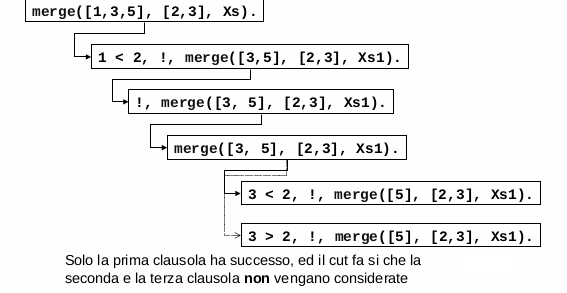
\includegraphics[scale=0.8]{img/cut3.png}
\end{center}
il programma del minimo diventa:
\begin{minted}{prolog}
minimum(X, Y, X) :- X =< Y, !.
minimum(X, Y, Y) :- Y < X, !.
\end{minted}
\textit{qui il secondo cut è ridondante ma viene messo per simmetria}.\\
Una volta che il programma ha fallito la prima clausola (ovvero il
test X =< Y) al sistema Prolog non rimane che controllare la
clausola seguente. Riscrivo in maniera non simmetrica:
\begin{minted}{prolog}
minimum(X, Y, X) :- X =< Y, !.
minimum(X, Y, Y).
\end{minted}
Qui si ha un red cut dato che taglia solo delle soluzioni, portando anche a risultati errati.\\
\subsection{Predicati Meta-Logici}
Vediamo il predicato:
\begin{minted}{prolog}
celsius_fahrenheit(C, F) :- C is 5/9 * (F - 32).
\end{minted}
Questo predicato non è invertibile. Si deve decidere qual è l'input e qual è l'output. Per questi problemi si hanno i \textit{predicati meta-logici}. La ragione di questo effetto (della non invertibilità) sta nell'uso che abbiamo fatto di vari predicati aritmetici nel corpo dei predicati (>, <, =<, is, etc), per poter usare i predicati aritmetici che usano direttamente l'hardware abbiamo sacrificato la semantica dei
nostri programmi.\\
I predicati meta-logici principali trattano le variabili come oggetti del linguaggio e ci permettono di riscrivere molti programmi che usano i predicati aritmetici di sistema come predicati dalla semantica “corretta” ed dal comportamento invertibile. Si hanno due predicati importanti:
\begin{itemize}
\item \textit{var(X):}  vero se \textit{X} è una variabile logica
\item \textit{nonvar(X):}  vero se \textit{X} non è una variabile logica
\end{itemize}
ovvero:
\begin{minted}{prolog}
?- var(foo).
No
?- var(X).
Yes
?- nonvar(42).
Yes
\end{minted}
il nostro programma dei gradi diventa:
\begin{minted}{prolog}
celsius_fahrenheit(C, F) :- 
	var(C), nonvar(F), C is 5/9 * (F - 32).
celsius_fahrenheit(C, F) :- 
	var(F), nonvar(C), F is (9/5 * C) + 32
\end{minted}
con var decido che clausola usare. L'uso di questi predicati ci permette di scrivere programmi efficienti e semanticamente corretti.
\subsection{Ispezione dei termini}
Posso chiedere a prolog se ho a che fare con termini atomici o scomposti, con i seguenti predicati:
\begin{itemize}
\item \textit{atomic(X): }vero se \textit{X} è un numero od una costante
\item \textit{compound(X):} vero se non \textit{atomic(X)}
\end{itemize}
Ho anche per manipolare un termine \textit{Term}:
\begin{itemize}
\item \textit{functor(Term, F, Arity)},
vero se \textit{Term} è un termine, con\textit{ Arity }argomenti, il cui funtore (simbolo di funzione o di predicato) è \textit{F}
\item \textit{arg(N, Term, Arg)},
vero se l’N-esimo argomento di \textit{Term }è \textit{Arg}
\item \textit{Term =.. L}
questo predicato, =..,viene chiamato (per motivi storici) \textit{univ}; è vero quando L è una lista il cui primo elemento è il funtore di \textit{Term} ed i rimanenti elementi sono i suoi argomenti
\end{itemize}
ovvero:
\begin{minted}{prolog}
?- functor(foo(24), foo, 1).
YES
?- functor(node(x, _, [], []), F, 4).
F = node
Yes
?- functor(Term, bar, 2).
Term = bar(_0,_1)
Yes
?- arg(3, node(x, _, [], []), X).
X = []
Yes
?- arg(1, father(X, lot), haran).
X = haran
Yes
?- father(haran, lot) =.. Ts.
Ts = [father, haran, lot]
Yes
?- father(X, lot) =.. [father, haran, lot].
X = haran
Yes
\end{minted}
\subsection{Programmazione di ordine superiore}
Quando si formula una domanda per il sistema Prolog, ci si
aspetta una risposta che è un'istanza (individuale) derivabile dalla knowledge base. Col backtracking ne abbiamo una alla folta, se le voglio tutte o voglio altri modi per acceder agli insiemi ho:
\begin{itemize}
\item \textit{findall(Template, Goal, Set):} 
\begin{itemize}
\item Vero se Set contiene tutte le istanze di Template che soddisfano Goal
\item \textit{Le istanze di Template vengono ottenute mediante backtracking}
\end{itemize}
\item \textit{bagof(Template, Goal, Bag):}
\begin{itemize}
\item Vero se Bag contiene tutte le alternative di Template che soddisfano Goal
\item Le alternative vengono costruite facendo backtracking solo se vi sono delle variabili libere in Goal che non appaiono in Template
\item È possibile dichiarare quali variabili non vanno considerate libere al fine del backtracking grazie alla sintassi $Var^G$ come Goal; In questo caso Var viene pensata come una variabile esistenziale
\end{itemize}
\item \textit{setof(Template, Goal, Set)}, che si comporta come bagof, ma Set non contiene soluzioni duplicate
\end{itemize}
\newpage
ovvero:
\begin{minted}{prolog}
/* findall */

?- findall(C, father(X, C), Kids).
C = _0
X = _1
Kids = [abraham, nachor, haran, isaac, lot, milcah, yiscah]
Yes.


/* bagof */

?- bagof(C, father(X, C), Kids).
C = _0
X = terach
KIDS = [abraham, haran, nachor];
C = _0
X = haran
KIDS = [lot, yiscah, milcah];
C = _0
X = abraham
KIDS = [isaac];
NO.

/* bagof con variabile esistenziale */

?- bagof(C, X^father(X, C), Kids).
C = _0
X = _1
Kids = [abraham, haran, lot, yiscah, nachor, isaac, milcah];
NO.
\end{minted}
\end{document}
